%---------------------------------------------------------------------------%
\lecture{Research Presentation}{lec_present_intro}
%---------------------------------------------------------------------------%
\section{\enorcn{Motivation}{引言}}%
%---------------------------------------------------------------------------%

\begin{frame}[fragile]
    \frametitle{Rayleigh B\'enard Convection}
    \begin{center}
        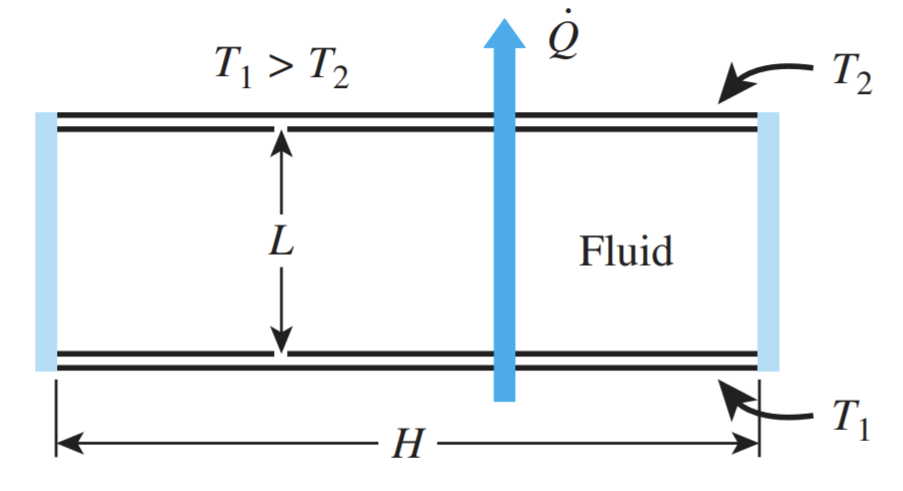
\includegraphics[width=8cm]{rbc_cengel.PNG}

        (Cengel 2015)
    \end{center}
\end{frame}

\begin{frame}[fragile]
    \frametitle{Why are we Still Studying Convection? \textbf{Applications}}
    \vfill
    % % \tikzart[t=m]{}% draw coordinate system
    % \tikzart[t=p,x=-6.3,y=-1.5,w=4]{earth-science-volcanoes-339345-1280x1024}{\fullcite{test}}% position picture
    % \tikzart[t=p,x=0,y=-1.5,w=4.2]{falk}% position picture
    % \tikzart[t=p,x=5,y=-1.5,w=4]{moto_fins}% position picture
    \begin{columns}
        \begin{column}{.30\textwidth}
            \centering
            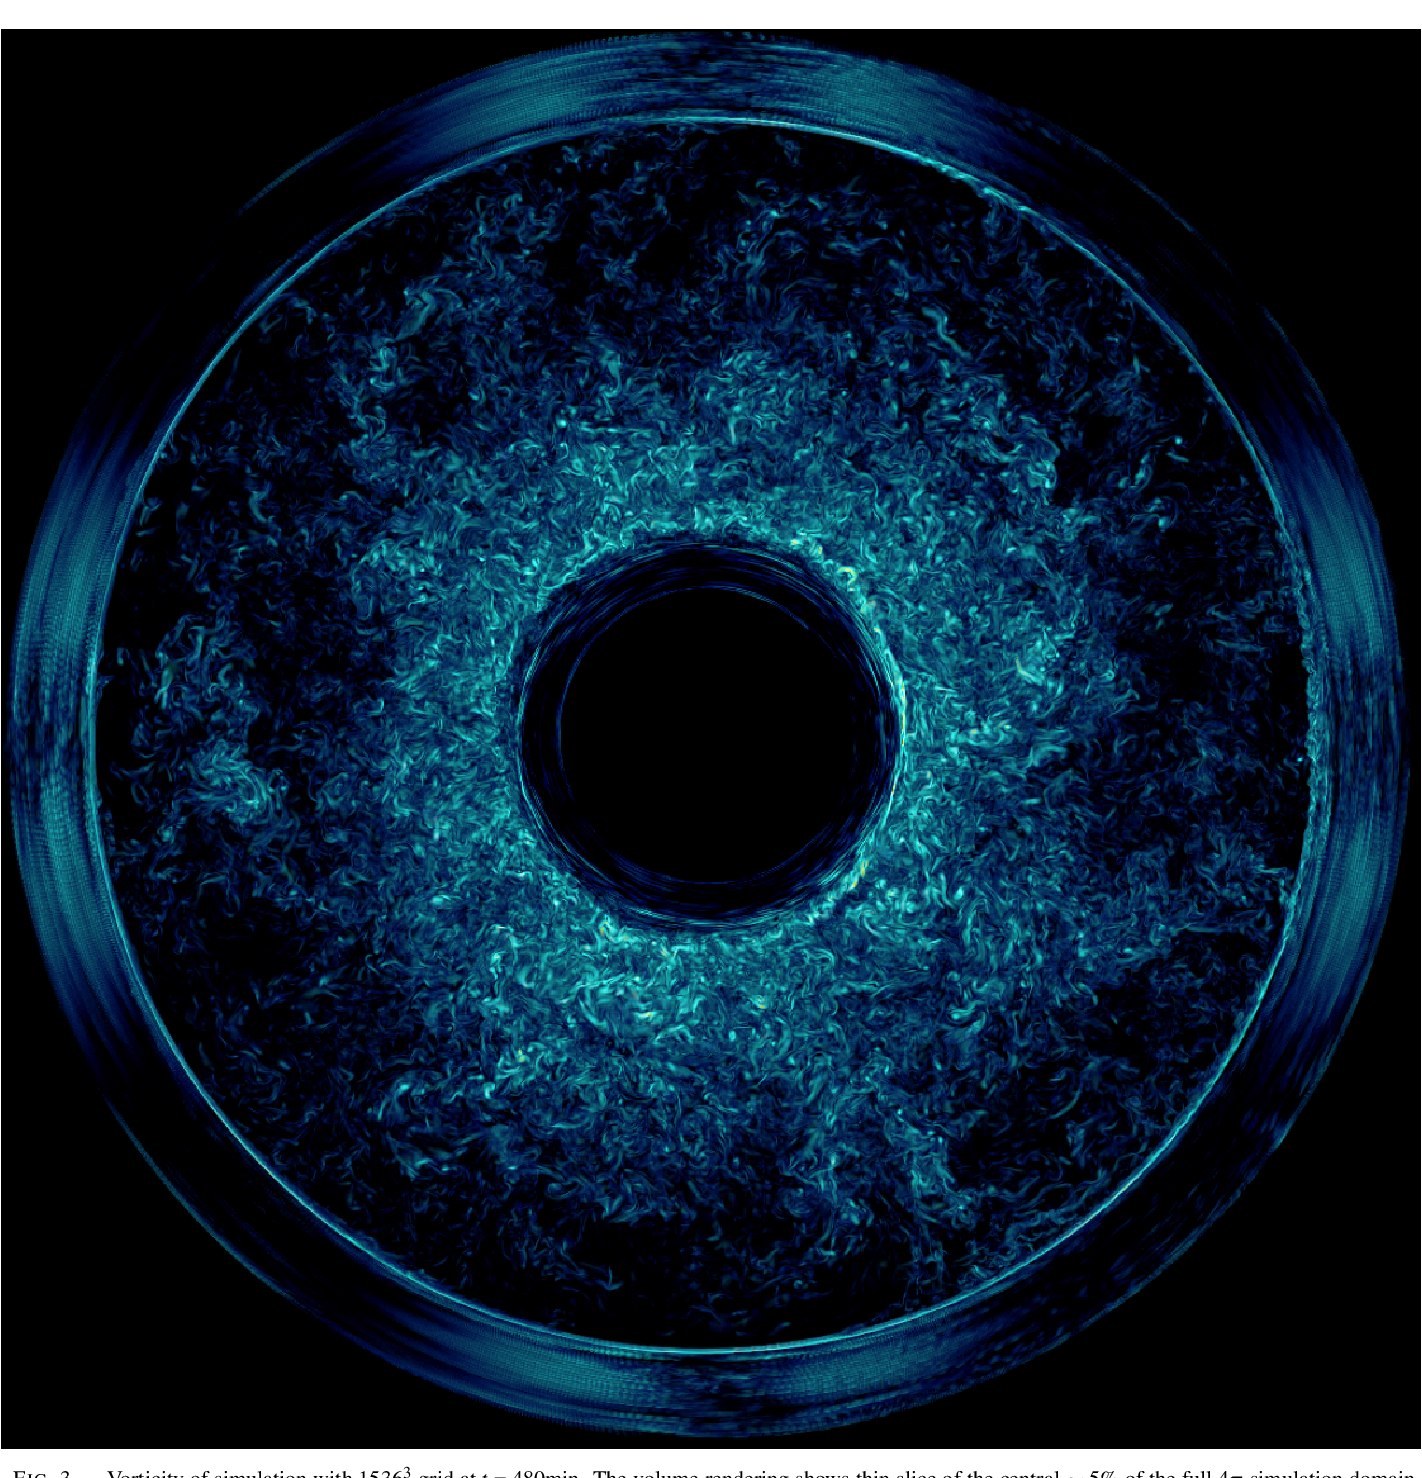
\includegraphics[height=0.8\textwidth]{falk.png}

            {Astrophysics}
        \end{column}

        \begin{column}{.3\textwidth}
            \centering
            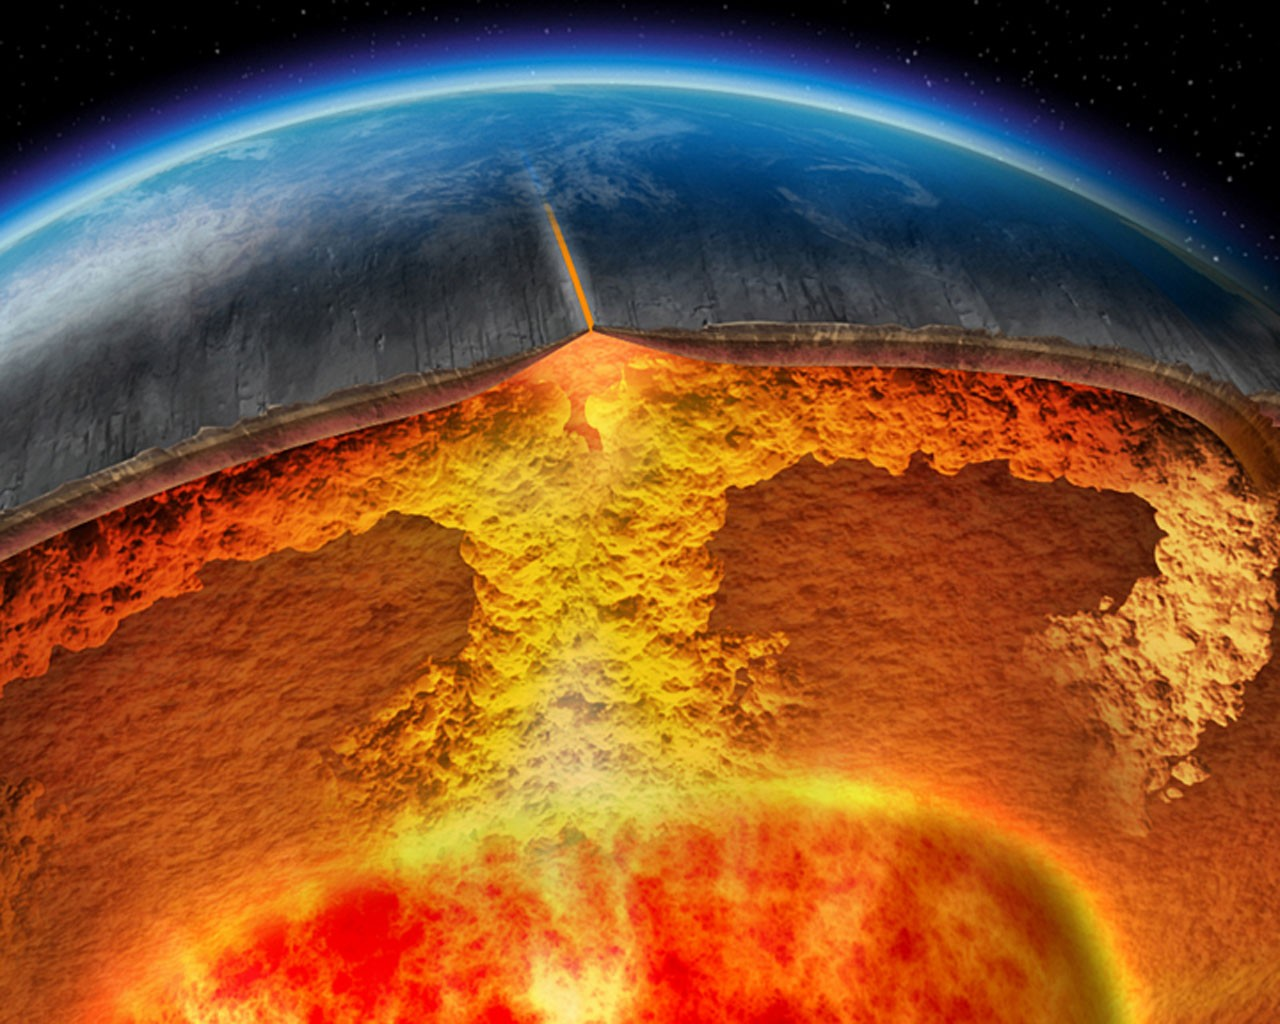
\includegraphics[height=0.8\textwidth]{earth-science-volcanoes-339345-1280x1024}

            {Geophysics}
        \end{column}

        \begin{column}{.30\textwidth}
            \centering
            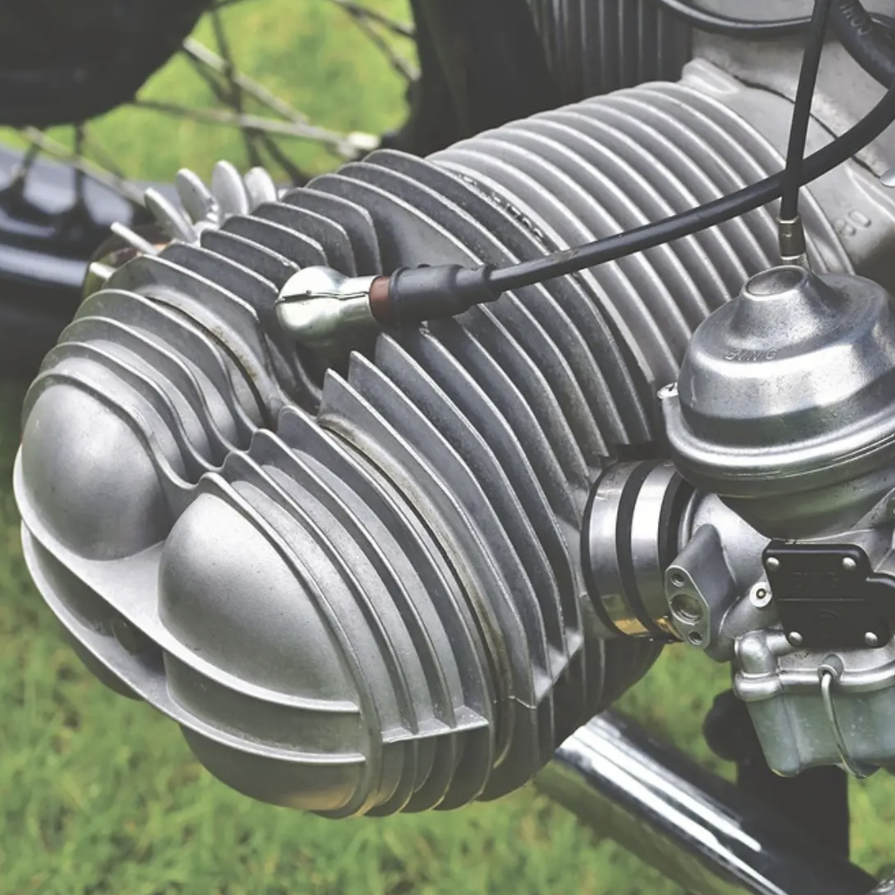
\includegraphics[height=0.8\textwidth]{moto_fins.png}

            {Engineering}
        \end{column}
    \end{columns}
\end{frame}

\begin{frame}[fragile]
    \frametitle{Why are we Still Studying Convection? \textbf{It's Elusive}}
    \vfill
    \begin{columns}
        \begin{column}{.30\textwidth}
            \centering
            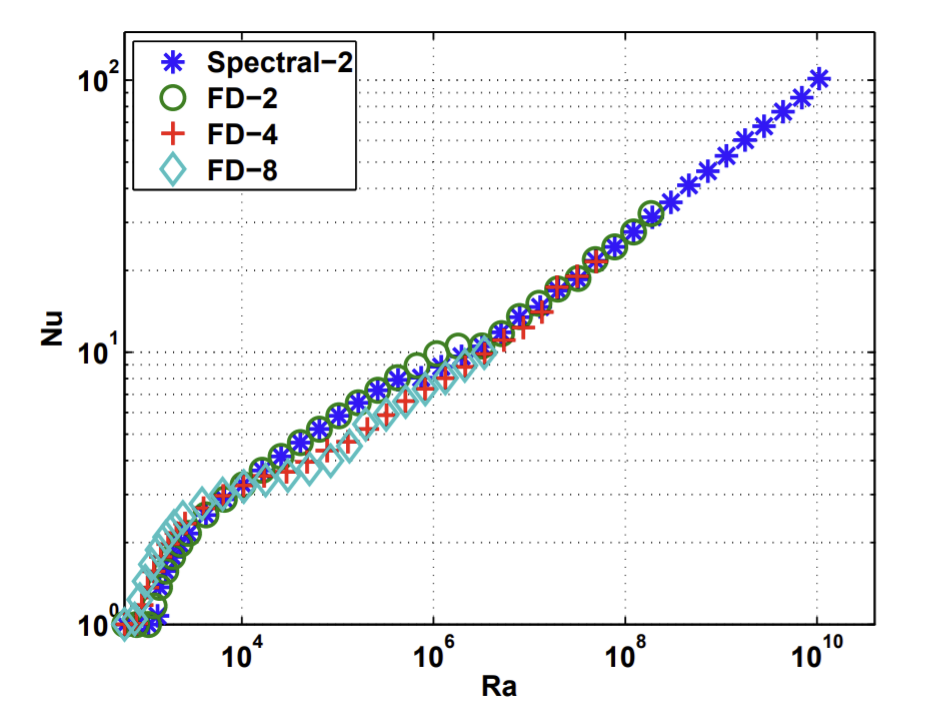
\includegraphics[height=0.85\textwidth]{johnson.png}

            {(Johnson and Doering 2009)}
        \end{column}

        \begin{column}{.60\textwidth}
            \centering
            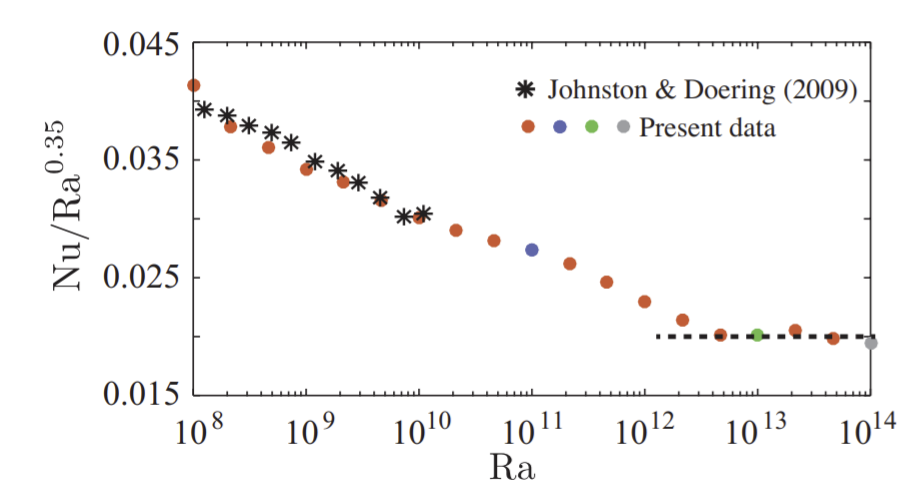
\includegraphics[height=0.5\textwidth]{zho.png}

            {(Zhu et al 2019)}
        \end{column}
    \end{columns}
\end{frame}

%---------------------------------------------------------------------------%

%---------------------------------------------------------------------------%
